% Created 2014-12-13 Sat 14:03
\documentclass[9pt,b5paper]{article}
\usepackage{graphicx}
\usepackage{xcolor}
\usepackage{xeCJK}
\usepackage{longtable}
\usepackage{float}
\usepackage{textcomp}
\usepackage{geometry}
\geometry{left=0cm,right=0cm,top=0cm,bottom=0cm}
\usepackage{multirow}
\usepackage{multicol}
\usepackage{listings}
\usepackage{algorithm}
\usepackage{algorithmic}
\usepackage{latexsym}
\usepackage{natbib}
\usepackage{fancyhdr}
\usepackage[xetex,colorlinks=true,CJKbookmarks=true,linkcolor=blue,urlcolor=blue,menucolor=blue]{hyperref}


\lstset{language=c++,numbers=left,numberstyle=\tiny,basicstyle=\ttfamily\small,tabsize=4,frame=none,escapeinside=``,extendedchars=false,keywordstyle=\color{blue!70},commentstyle=\color{red!55!green!55!blue!55!},rulesepcolor=\color{red!20!green!20!blue!20!}}
\author{Jenny Huang}
\date{\today}
\title{Android App Programming Directed Study \textasciitilde{} DrawingFun}
\hypersetup{
  pdfkeywords={},
  pdfsubject={},
  pdfcreator={Emacs 24.3.1 (Org mode 8.2.7c)}}
\begin{document}

\maketitle
\tableofcontents


\section{first checkin 10/27/2014}
\label{sec-1}
\subsection{Goal}
\label{sec-1-1}
\begin{itemize}
\item According to the instructor's requirements that we are going to implement an simple window's Paint like Android app for later on integrating Unicon's 2D graphics to Android app.
\end{itemize}
\subsection{Course Introduction}
\label{sec-1-2}
\begin{itemize}
\item We have only two students, the other one is an udnergraduate exchange students with solid Java programming background and relatively slightly week problem-solving skills. For the first more than half semester, we used Sudoku as the starting point and tried several different topics to get our hands wet.
\end{itemize}
\subsection{Project Introduction}
\label{sec-1-3}
\begin{itemize}
\item It's after middle term already, the way we were currently trying on to make it work may just work perfectly for the other classmate, but for me, I feel like it takes forever for me to be able to make any significant progress. So about half a month ago, I was motivated and thought instead of surfacing around and having fun learning by trial and error, maybe I should start from an simple GUI app as a starting point and try my best to expend/extend the APP functionality from there. And also we would be able to work to our final project slightly earlier.
\item This GUI will be my very second GUI interface that I have ever created for my Computer Science major, (this first one was an Python Tkinter GUI one week short project for plotting graphics with data abstracted from backend database during an internship;). And I guess it may still be slightly difficult for me to start write Android App code of my own line by line, so I simply searched internet, and trying an tutorial to make a working starting point Android Paint GUI. I integrated the codes from the reference link all together, fixed minor compile errors, and it worked!
\item This "Copied" GUI will serve as the starting point, and my functionality updates start from here, and I will update my progress for this project later on by week according to the instructor's requirements and suggestions.
\end{itemize}
\subsection{References}
\label{sec-1-4}
\begin{itemize}
\item \url{http://code.tutsplus.com/tutorials/android-sdk-create-a-drawing-app-interface-creation--mobile-19021}
\end{itemize}
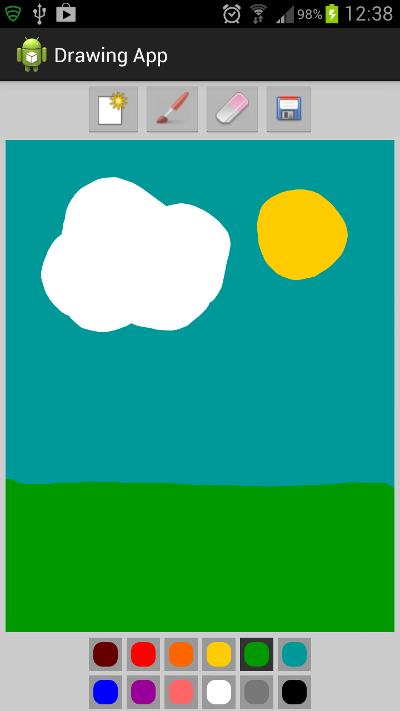
\includegraphics[width=.9\linewidth]{./android_drawing_final.png}

\section{Checkin for 11/3/2014}
\label{sec-2}
\subsection{Buttons I have worked on}
\label{sec-2-1}
\subsubsection{Color$_{\text{Picker}}$:}
\label{sec-2-1-1}
\subsubsection{Undo/Redo:}
\label{sec-2-1-2}

\subsection{Functionalities and References}
\label{sec-2-2}
\subsubsection{Color$_{\text{Picker}}$:}
\label{sec-2-2-1}
\begin{itemize}
\item Motivated by the Picasso Android app, seeing their multiple color choices, our starting point \textbf{12} fixed colors were too limited.
\end{itemize}
\subsubsection{Undo/Redo Buttons:}
\label{sec-2-2-2}
\begin{itemize}
\item Also motivated by the Picasso app, intended to work on \textbf{Undo} button, and ended up found \textbf{Redo} button could be very convenient as well.
\item needs to update these Undo/Redo methods later on, this is just the starting point most basic implementation for this button set.
\end{itemize}
\subsection{Snapshot}
\label{sec-2-3}
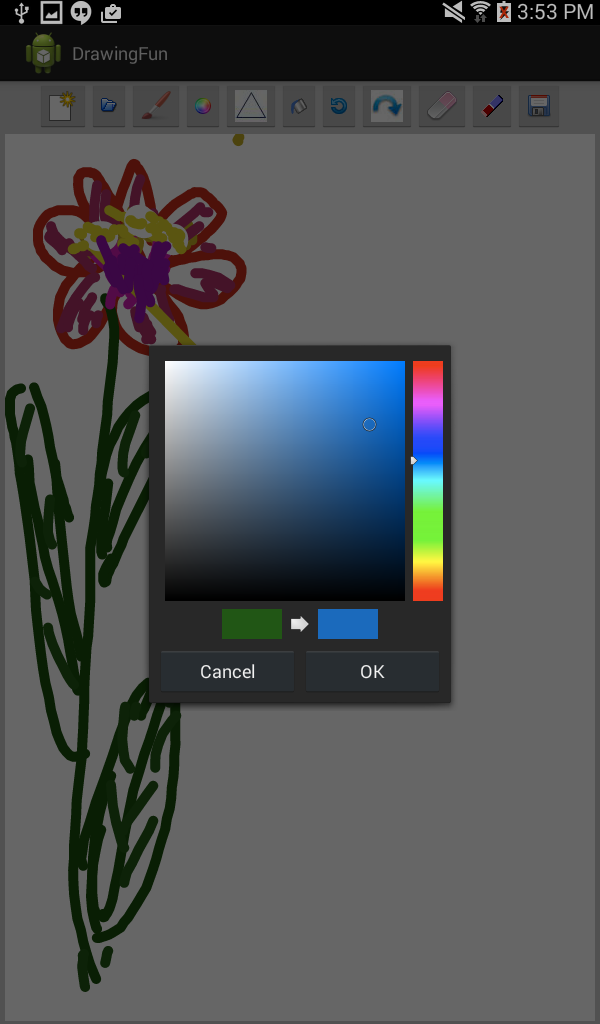
\includegraphics[width=.9\linewidth]{./20141103.png}

\subsection{Todo}
\label{sec-2-4}
\subsubsection{Drawing shapes with Finger for primitives}
\label{sec-2-4-1}
refer to the reference below: 
\begin{itemize}
\item \url{http://gmariotti.blogspot.com/2014/01/drawing-shapes-with-fingers.html}
\item This button will be first priority to finish
\end{itemize}
\subsubsection{Load image file button}
\label{sec-2-4-2}
\subsubsection{Erase Rectangle}
\label{sec-2-4-3}
\subsubsection{Undo/Redo}
\label{sec-2-4-4}
\section{Checkin for 11/10/2014}
\label{sec-3}
\subsection{Buttons I have worked on}
\label{sec-3-1}
\subsubsection{shapeBtn for primitives}
\label{sec-3-1-1}

\subsection{Functionalities and References}
\label{sec-3-2}
\subsubsection{shapeBtn for primitives: Drawing shapes with Finger for primitives}
\label{sec-3-2-1}
\begin{itemize}
\item refer to the reference below for some basic shapes: line, smooth line, circle, triangle, Rectangle, square
\item \url{http://gmariotti.blogspot.com/2014/01/drawing-shapes-with-fingers.html}
\item \textbf{ListView} in \textbf{Alert Dialog} is searched from online without direct reference.
\item Since the erase was using draw smooth line. This button works also means that I could erase a "\textbf{Rectangle}" shape, or "\textbf{Circle}" shape.
\item I have other course priority for the passed week, so I just have enough time to finish this course's priority, but I will try to work harder in order to finish all the functionalities for this course.
\item It's not a good looking ListView, but yet it's a fully functional button.
\item This button right now is fully functional, but to finish this project first, I have not spent any quality time to expand any primitives yet, rather than the existing six ones from the reference listed below.
\end{itemize}
\subsection{Snapshot}
\label{sec-3-3}
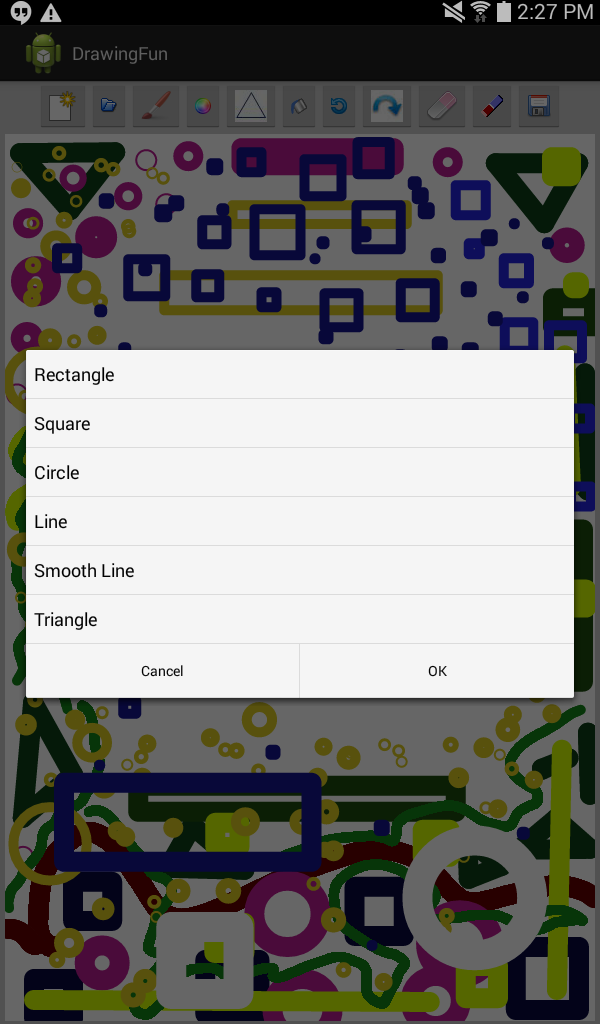
\includegraphics[width=.9\linewidth]{./20141110-14-27-05.png}
\subsection{Special Situation}
\label{sec-3-4}
\begin{itemize}
\item There were too many students piled/lined up in front of Dr. Jeffery's door, and he didn't break the line by stating that it's our direct study time. So the other classmate and I just stepped away from his office, and we didn't really meet during last week.
\item The other classmate and I have talked, and we happened to have worked on the same shapeBtn, I applied ListView in a dialog box with all six drawing shapes applied, and he created a (ListView? not sure) with a clickable button as one element with four shapes applied. And he agreeed my ListView looked way prettier than his buttons did.
\item But I am willing to and more than happy to think that he could have worked on something else important for him that I actually didn't have time to work on during the passed week.
\end{itemize}
\subsection{Todo}
\label{sec-3-5}
\begin{itemize}
\item Load image file button
\item Erase Rectangle
\item Undo/Redo
\item Fill paint
\end{itemize}

\section{Checkin for 11/17/2014}
\label{sec-4}
\subsection{Buttons I have worked on}
\label{sec-4-1}
\begin{itemize}
\item openBtn for loading an image file as an ImageView
\item Undo/Redo
\end{itemize}
\subsection{Functionalities and References}
\label{sec-4-2}
\subsubsection{openBtn for loading an image file as an ImageView}
\label{sec-4-2-1}
\begin{itemize}
\item The method I applied is memory saving for AsyncTask, which is better than load images directly, which could potentially block UI for couple of seconds;
\item Loaded an image from online, but would like to try load internal images from device later on, like a drawing which I saved earlier onto my internal device;
\item Potentially apply layer oncepts to produce multiple layer drawing, needs suggestions to organize my idea how to implement this feature.
\item \textbf{Question}: Right now, my image is an ImageView in my layout, what ideas that I could use to set/change/transfer my ImageView to be my draw view background?
\item References:

\url{http://www.learn2crack.com/2014/06/android-load-image-from-internet.html}

\url{http://stackoverflow.com/questions/5776851/load-image-from-url}

\url{https://github.com/koush/UrlImageViewHelper}
\end{itemize}

\subsubsection{Undo/Redo}
\label{sec-4-2-2}
\begin{itemize}
\item After implemented subclass SuperActivity class which extends Activity on week checkin for 11/10/2014 for my ListView implementation, subclass of Path() was very difficult for me to think about implement before, but after my trial on ListView, super/sub class in Java all made sense to me now. It's a piece of cake, and I know I can wrap whatever material I need in order to paint nice and neat.
\item Implemented by developing a subclass myPath to wrap the super Path(), drawPaint color, and drawPaint strokesize together as an object.
\item Based on previous progress that I can undo/redo only with all the drawCanvas with the same paint color, now my updo/redo paths could be colorful and with various strokesizes.
\item References:

Path() library:

\url{http://grepcode.com/file/repository.grepcode.com/java/ext/com.google.android/android/2.3.1_r1/android/graphics/Path.java}

Bitmap cacheing:

\url{http://stackoverflow.com/questions/3406910/efficient-2d-drawing-in-android/3408641#3408641}

\item \textbf{Questions}: 

\begin{enumerate}
\item Undo/Redo for simple path seem to behavor fairly ok, but instead of lineTo wired line, how do I implement smooth line? How could I differentiate different strokesizes more clear with lines I have so far?

\item One little detail though, I dras after touch up, my paint color change delayed, how do I implement \textbf{real time}?

\textbf{Answered}: drawPath.reset() produced all the trouble.

\item About previous ListView six different shapes, with Undo/Redo properly functionaing, I realize I just lost my siz shapes again cause I need to rewrite/implement methods in order for them to be able to Undo/Redo \textasciitilde{}? (My subclass works perfectly for this propose, just that I lost my internal link to primitives, which means I probably should rewrite my primitives draw methods according to undo/redo prerequirements. I don't think it will be difficult, but I don't have enough time for this for the pass week, and I need to organize my ideas about these implementation clear. )

\item I prioritize undo/redo to be more important than any other buttons cause I know they would give me great practise together with primitives implementation methods rewrite. So I have not touch "Erase Rectangle" button and "paint fill" button yet. According to these idea, I would prioritize Rectangle rewrite with the highest priority, so that later on I can follow up with erase Rectangle (which means draw Rectangle first, fill with background color, and undo could remove this erase step). Correct me if I am wrong.
\end{enumerate}
\end{itemize}

\subsubsection{References: all about Android}
\label{sec-4-2-3}
\begin{itemize}
\item \url{https://github.com/kesenhoo/android-training-course-in-chinese}
\end{itemize}

\subsection{Snapshot}
\label{sec-4-3}
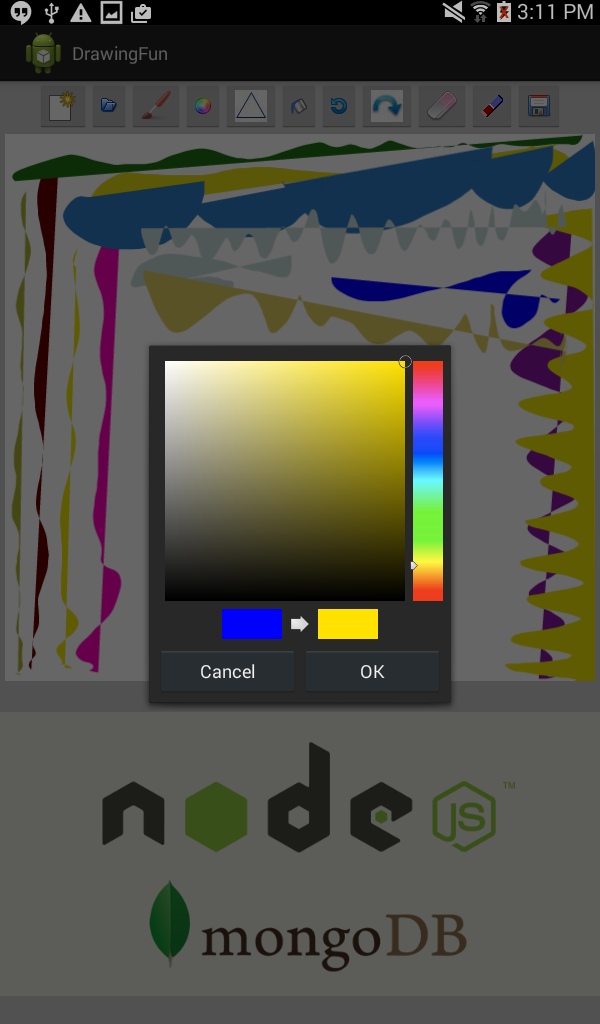
\includegraphics[width=.9\linewidth]{./Screenshot_2014-11-17-15-11-20.png}
\subsection{Todo}
\label{sec-4-4}
Only two button left untouched, could do the following or anything I am interested to implement. 
\begin{itemize}
\item Erase Rectangle
\item Fill paint
\end{itemize}

May try to \textbf{save} into Galaxy\ldots{} as Dr. Jeffery mentioned it last time when we meet during class;

Potential interests: may implement depends on how I spend thanksgiving \textasciitilde{}~
\begin{itemize}
\item touch ImageView Activities: zoomin, zoomout, rotate, fading, etc
\item SurfaceView rotate images through new thread
\item canvas save() and restore()
\item OpenGL spinning circle
\item widely used draw methods
\item Easy draw operations
\end{itemize}

\section{Checkin for 12/01/2014}
\label{sec-5}
\subsection{Buttons I have worked on}
\label{sec-5-1}
\begin{itemize}
\item ImageView to Bitmap
\item start newBtn
\item Undo/Redo
\end{itemize}
\subsection{Functionalities and References}
\label{sec-5-2}
\subsubsection{ImageView to Bitmap}
\label{sec-5-2-1}
\begin{itemize}
\item Worked on Bitmap so that I can load a picture as my drawView background;
\item This could be considered to be a trial, and could try to add user options to different background pictures later on;
\end{itemize}
\subsubsection{start newBtn}
\label{sec-5-2-2}
\begin{itemize}
\item Realized that my newBtn lost its functionality during last checkin because of different mechanisms, and I fixed it after having implemented undo/redo for paths;
\item The wired drawing path shapes (like the dramatic curves in previous Snapshot) got corrected as well by writing to Bitmap;
\item References: mutuable immutable bitmaps 

\url{http://stackoverflow.com/questions/13119582/android-immutable-bitmap-crash-error}
\item But I still failed to start new because some minor error about implementation. I uninstalled the app and restart, the error was still there;
\item I was so focused on the mview thing that I completely lost focus on the true reason. Once I asked and the instuctor helped explain that invalidate() simply calls onDraw() function, I could immediately realize that I forgot to clean my undo/redo arraylist paths and undonePaths!
\item It was the invalidate() function confused and prevented me from relaxing on the mview, and I was stubborn there for about one hour this afternoon. Realizing that I felt so sorry for myself for the one hour being so stupid! And right now I am on my way following the good habit reading Qt creator documents systematically before googling the correct answer only when I try to solve my technical difficulties, which is good.
\item While it still worths a minutes to rewind and rethink about what happened during that one hour, how I trusted myself so much and suspected on low probability corner cases situations, rather then double check and confirm that all the steps/processes I had made were correct and reliable. I wished I spend the hour with a scientific attitude the latter.
\end{itemize}
\subsubsection{Undo/Redo}
\label{sec-5-2-3}
\begin{itemize}
\item If I really don't want to separate/pack my ListView items into objects, will it be possible for me to use command pattern instead, and how difficult could command pattern to be comparatively spearking?
\item References:
List: 
\begin{itemize}
\item \url{http://stackoverflow.com/questions/11114625/android-canvas-redo-and-undo-operation}
\end{itemize}
Command Pattern:
\begin{itemize}
\item \url{http://www.28im.com/android/a141932.html}
\item \url{http://www.javaworld.com/article/2077569/core-java/java-tip-68--learn-how-to-implement-the-command-pattern-in-java.html}
\item \url{http://www.28im.com/android/a141932.html}
\item \url{http://blog.csdn.net/lovingprince/article/details/1532869}
\item \url{http://www.2cto.com/kf/201409/333267.html}
\item \url{http://www.2cto.com/kf/201406/309574.html}
\item \url{http://blog.csdn.net/rhljiayou/article/details/7212620}
\end{itemize}
\item Answers: 
\begin{itemize}
\item We didn't really talk about command patterns at all this afternoon, but rether to solve both the other classmate's and my technical difficulties, and also discussions about the questions we raised, for example, my interested ones including multiple layers Potentials when using Bitmap and removing any layers afterwards, and autosave nsapshots if we save bitmap every 20 minutes, and Potential values we could apply with those save displays in paths \& undonePaths during each 20 minoutes interval.
\item I began to realize that I COULD have my own little brain-turning/intuitive ideas when I began to understand things, like I spent hours today just to understand Bitmap\textasciitilde{}
\end{itemize}
\end{itemize}
\subsection{Snapshot}
\label{sec-5-3}
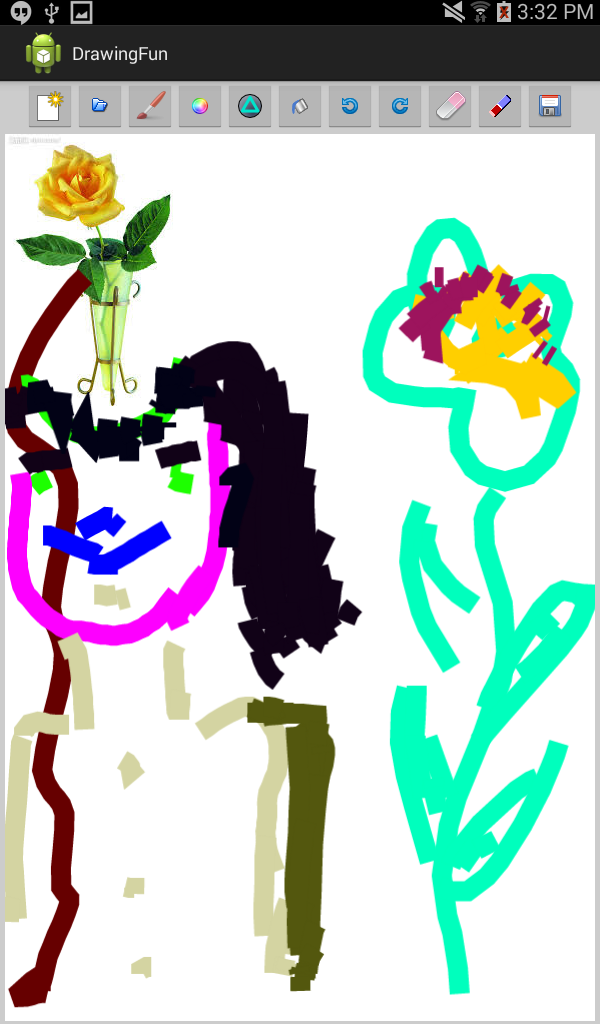
\includegraphics[width=.9\linewidth]{./Screenshot_2014-12-01-15-32-21.png}
\subsection{Todo}
\label{sec-5-4}
\begin{itemize}
\item finish the undone functions and wrap up project and do basic demo on coming Monday;
\item short about one page summary, could at most to be 2 pages;
\end{itemize}

\section{Checkin for 12/08/2014}
\label{sec-6}
\subsection{Buttons I have worked on}
\label{sec-6-1}
\begin{itemize}
\item Undo/Redo
\item Erase Button
\item FloodFill
\end{itemize}
\subsection{Functionalities and References}
\label{sec-6-2}
\subsubsection{Undo/Redo}
\label{sec-6-2-1}
\begin{itemize}
\item \textbf{Cleaned} my contamination or origial bitmap in DrawView \textbf{clear()} method by replacing "new2Bitmap = originalBitmap; " with "new2Bitmap = bridgeBitmap.copy(Bitmap.Config.ARGB$_{\text{8888}}$, true);"
\item I used bitmap only for the propose of adding the Yellow Rose which I liked it too much and wanted to keep it as a corner backgroung; But for the rest of drawings, they are all drawn on canvas instead of bitmap;
\item I could draw all the contents in bitmap, but my \textbf{Straight Line} looked really wired on bitmap when I draw in progress, but otherwise I don't have any clear idea how to remember the start and end points and draw a straight line during onDraw. I need some idea here, if I continued to use bitmap instead of canvas;
\item Fixed minor issue for smooth line undo when I tried the function onSizeChange, which was originally working before;
\end{itemize}
\subsubsection{Erase button}
\label{sec-6-2-2}
\begin{itemize}
\item Becuase I liked the Yellow Rose too much, I had to conpensate and rewrite the erase function to draw shapes using background color, because the old method doesn't work any more when I used bitmap; The function itself was not difficult at all though.
\end{itemize}
\subsubsection{FloodFill}
\label{sec-6-2-3}
\begin{itemize}
\item Implemented on Bitmap instead of canvas
\item I used bitmap only for the propose of adding the background image and do the FloodFill on the background image. But for the rest of drawings, they are all drawn on canvas instead of bitmap;
\item Applied the following method, but it was way too slow, and look urgyly
\item \url{http://stackoverflow.com/questions/12669740/android-using-flood-fill-algorithm-getting-out-of-memory-exception}
\item \url{http://stackoverflow.com/questions/8070401/android-flood-fill-algorithm}
\item \url{http://www.codeproject.com/Articles/364413/Queue-Linear-Flood-Fill-A-Fast-Flood-Fill-Algorith}
\item \url{http://stackoverflow.com/questions/8723590/fill-the-complete-canvas-but-keep-the-bound-fill-area-as-it-is-like-circle-rect/12777805#12777805}
\item \url{http://blog.csdn.net/jia20003/article/details/8908464}
\end{itemize}
\subsubsection{Other Issues}
\label{sec-6-2-4}
\begin{itemize}
\item setBrushSize 
\begin{itemize}
\item Issue: the setBrushSize option always changed the drawView color back to initial default color, which is Color.BLUE, and which is not convenient;
\item In \textbf{MainActivity}, when draw$_{\text{btn}}$ I setBrushSize, I have to do \textbf{drawView.setColor(mColor);}, otherwise, it always set drawView's paintColor to be default Color.BLUE;
\item But I don't think the above implementation is logical. I don't think click on draw$_{\text{btn}}$ need to do anything about color when I suppose to set the brushSize; But I have difficulties to understand the process and find a better "logical" solution for it.
\end{itemize}
\item onSizeChange
\begin{itemize}
\item I think I have bug on \textbf{onSizeChange} function, because whenever I changed my device from vertically to horizontally, all the contents on my canvas just went away.
\item I can think the reason is because I didn't really draw anything on the bitmap yet, and that's the reason whenever I changed from vertical to horizontal, I have only my fresh loaded background bitmap;
\item But, if I want to draw on bitmap, I will have to reimplement my undo/redo differently, the current ArrayList method won't work any more.
\item If I reimplement on bitmap, what will be the good idea to implement it?
\item I would be happy if the instructor helps Introduce a little bit more 0about bitmap, undo/redo on it, and its utilities.
\end{itemize}
\end{itemize}
\subsubsection{report}
\label{sec-6-2-5}
\begin{itemize}
\item Course report is in \textbf{report.org} file, and main sections are also copied into the followed section for the reader's convenience.
\item The demo was reviewed today and the course is done. I did pretty good job for this DrawingFun project and the course, but I need to prioritize my tasks, and I won't be able to update this repository for a while. Thanks for looking.
\end{itemize}
\subsection{Snapshot}
\label{sec-6-3}
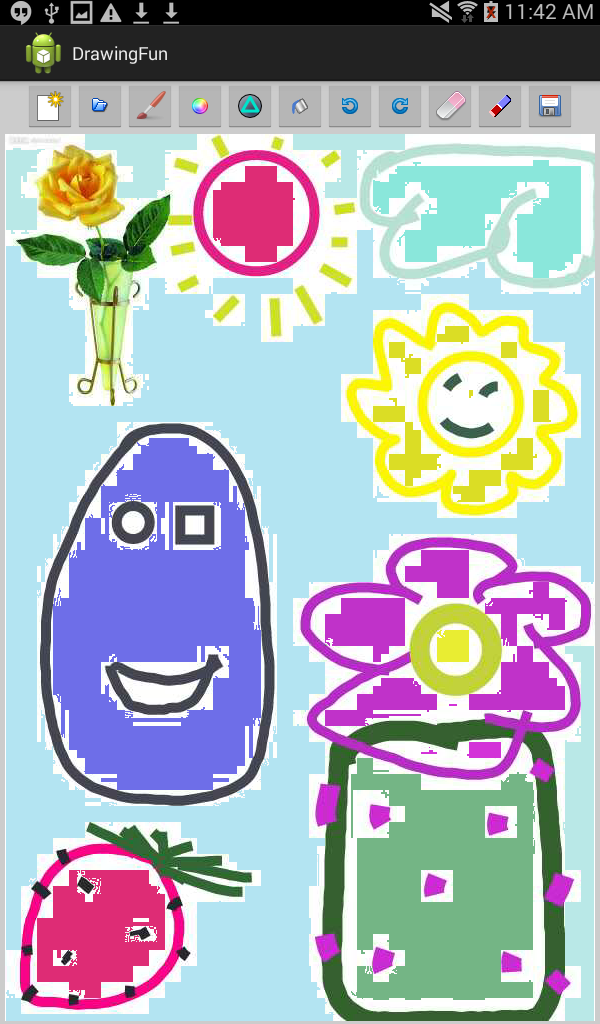
\includegraphics[width=.9\linewidth]{./Screenshot_2014-12-08-11-42-04.png}

\section{Course Review}
\label{sec-7}
\subsection{Course Goal and General Review}
\label{sec-7-1}
\begin{itemize}
\item Taking this course, I wanted to help myself stay on schedule and learn some cutting-edge knowledge as a starting point.
\item I never had any "new" knowledge like "Android" learned before, this is the first time, and I enjoy it;
\item I enjoyed two modules the most: the color popup dialog and undo/redo functionalities. And in the middle, ListView helped a little bit as well;
\begin{itemize}
\item The color picker was not my original work, but for me at that time, it was very complicated and it forced me to understand all the Android framework for an App to function, the manifest, layout, value etc;
\item To implement a fully functional ListView together with the rest functionalities, I figured out my own way of creating a bridge SuperActivity class, which in term of Java-programming, created a start point of confidence that I can implement my ideas (any idears) in Java as far as I \textbf{Think} it through, clear. \textbf{It is always the ideas that matter, instead of any implementation.}
\item For undo/redo interface/implementation, I had thought to skip around by implementing Command Patterns, but now I am glad that Dr. Jeffery insisted us to apply interface/implementation. And I had been frustrated yet more than happy take my own effort to try, step by step, implement and see eventually it is working\textasciitilde{}! And during this process, I felt I began to be exposed to Java OOD, Android canvas, bitmap, drawing primitives, and I understood the theory behind them now, even only the parts that I implemented.
\end{itemize}
\end{itemize}
\subsection{Course Benefits}
\label{sec-7-2}
\begin{itemize}
\item The latter half semester of implementing DrawingFun Paint project helped me realize that I can perform great in concentrated topics, which helps me focus.
\item It has been a challanging and interesting learning experience during this Android App Programming, and it successfully reached the target which I expected from this course. I learned the basic necessary knowledge to build my Android App and Java Programming background, and I practised and cultivated the necessary and usefull skills to think logically, solve problems and debug my codes.
\item The course built knowledge, practised skills, as well as built confidence in programming and problem-solving, and help cultivated my \textbf{I CAN DO} attitude towards projects.
\item After taking this course, I have a sufficient starting point to self-learn and practise Android App Programming. And now I am ready to prefer Java over c++ as my primary and first choice programming language, and I will try to conduct more practise on Java programming so I can be proficient on it in not far future.
\end{itemize}
\subsection{Report Feedback from Instructor - 12/12/2014}
\label{sec-7-3}
\begin{itemize}
\item I got the report feedback from the course instructor today that he doesn't require any coding work any more as was concluded on Monday's demo and review already, but he would still expect a slightly better version of report from me with the marked requirements;
\item A scann copy of my origial report and the course instructor's marks are attached below, and I will make necessary modifications for it so it satisfies his requirements.
\end{itemize}
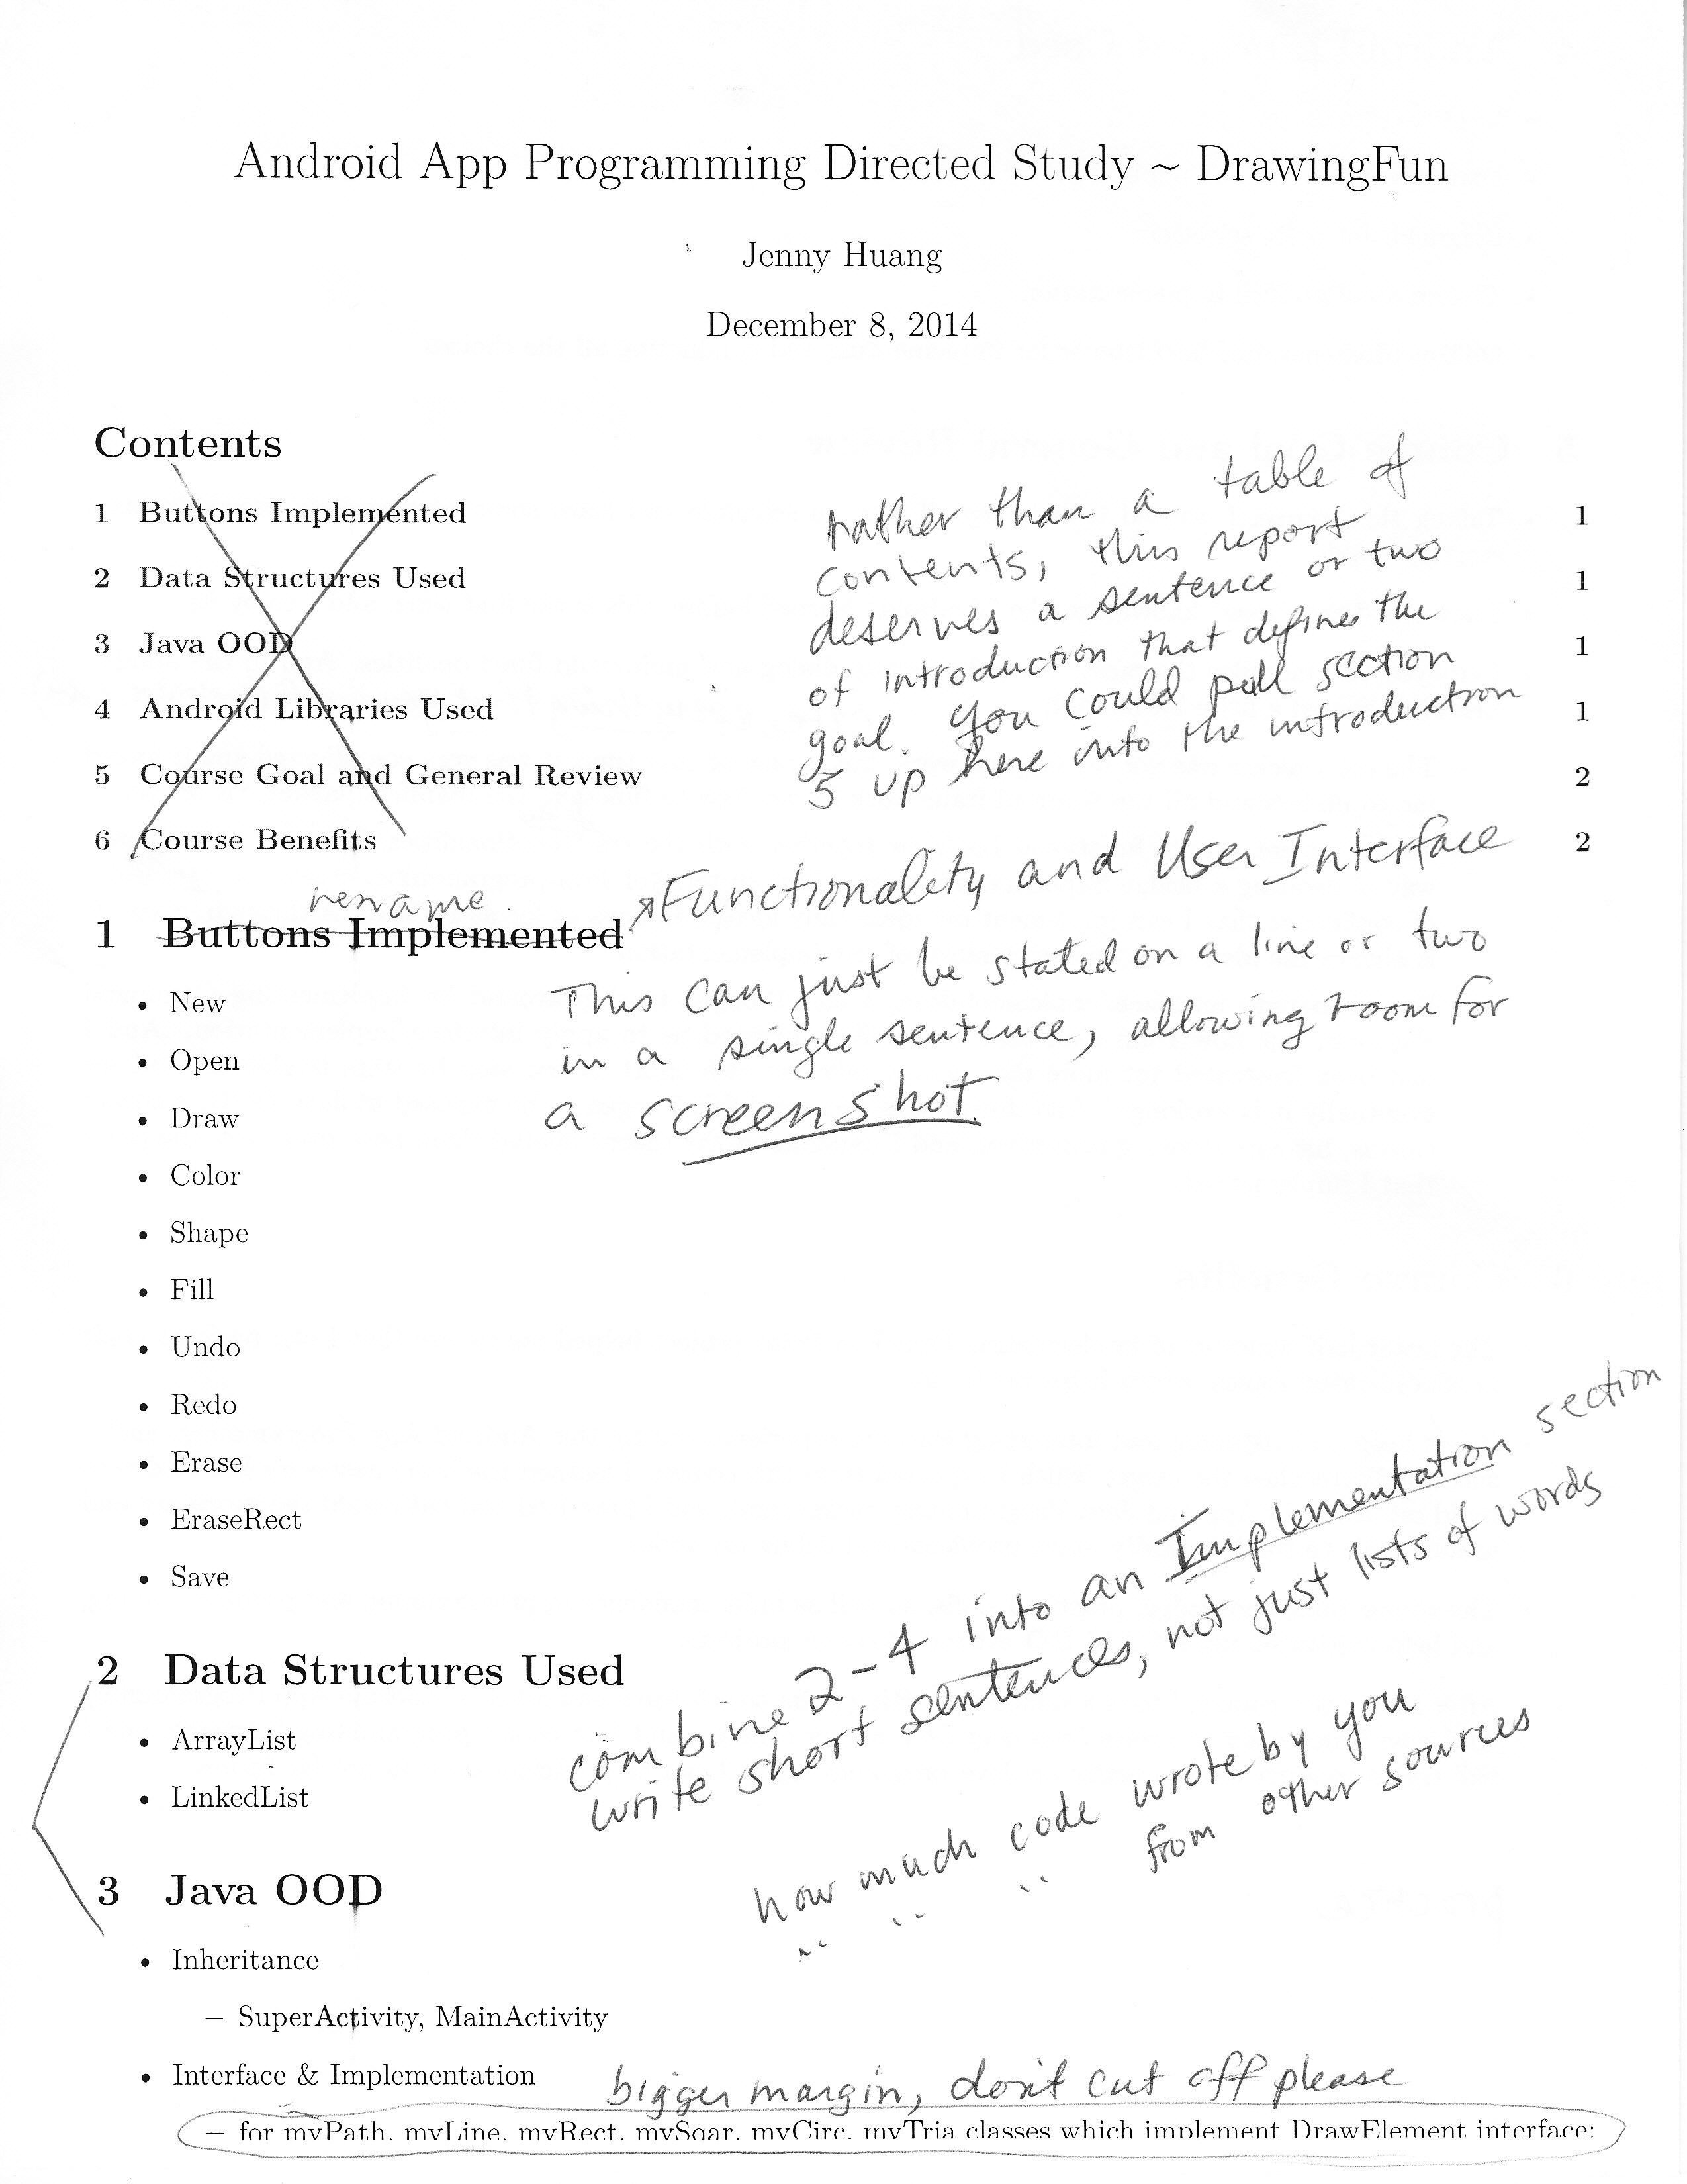
\includegraphics[width=.9\linewidth]{./IMG_0001.jpg}

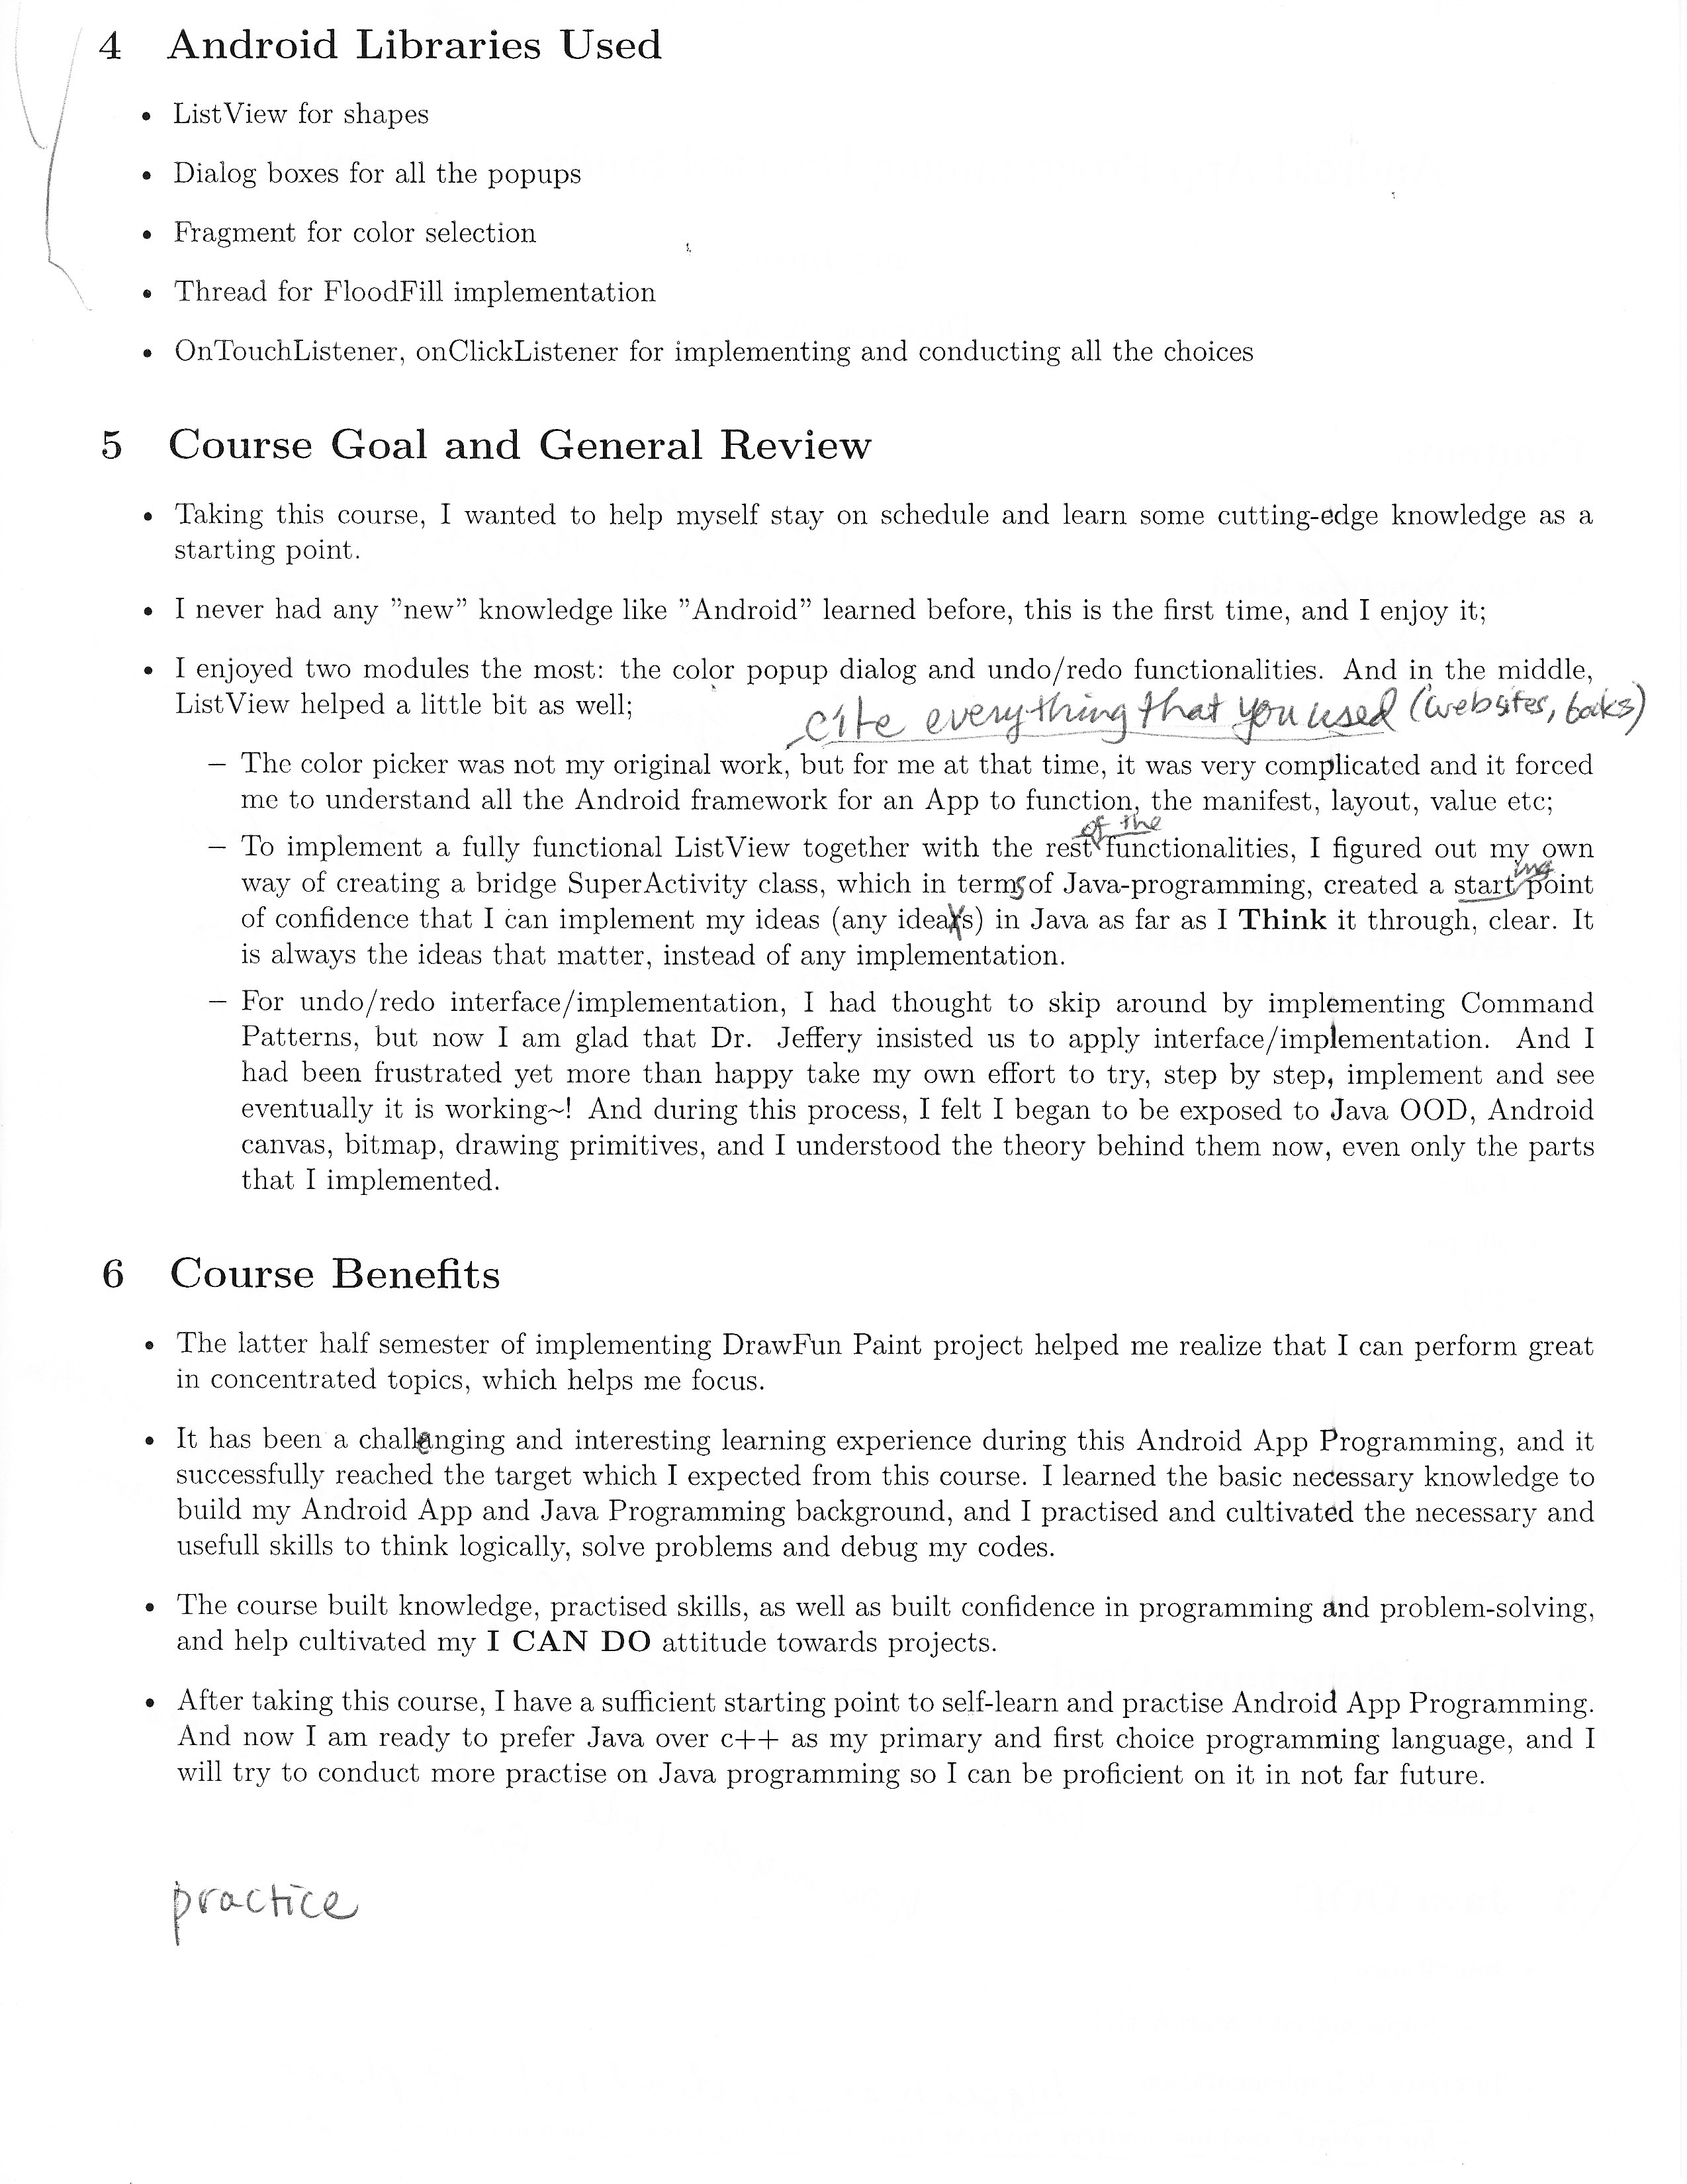
\includegraphics[width=.9\linewidth]{./IMG_0002.jpg}
\begin{itemize}
\item The final report deadline for me is Friday, coming week. Of course I would be able to finish on time. I will update this repository when I finish my updated report as well.
\end{itemize}
\subsection{practice vs practise}
\label{sec-7-4}
\begin{itemize}
\item When I knoced the door of my instructor's office yesterday (12/12/2014, \textbf{now I am modifying on 12/13/2014}) at noon, the instructor said he was right on working on my report, and if I could wait several minutes, he would be able to finish. So I waited in his office, and he searched internet on propose that the \textbf{practise} in my last section should be writen as \textbf{practice}, and that was the reason he wrote \textbf{practice} on my second page.
\item And after he searched the word using google, he emphasized by talking to me that in bratish english, people may spell \textbf{practice} as \textbf{practise}, but in America, they use to write as \textbf{practice}. He wrote the word down on my report without circling the original wrong-spelled word.
\end{itemize}

\section{Personal Conclusion}
\label{sec-8}
\begin{itemize}
\item I had minor difficulties setting up my Android environment at the beginning of the semester, like my window's SDK manager never worked; And at the beginning of the semester my Linux Mint 17 Eclipse kept crashing\ldots{} It was from time to time, I searched and googled, and get my Linux version stable; And I did have some help from the other classmate as well;
\item The first half semester kind of, the course contents were slightly distributed, and I felt I didn't really know what to focus, and I don't like that half of semester;
\item The rest about half semester I worked on this DrawingFun project, and I am confident that I did pretty good job, comparatively spearking, compared with the other classmate. 
\begin{itemize}
\item I applied Color-Picker functionality, while he applied mine;
\item I applied ListView for drawing primitives, while he applied the same original setting-brush-size methods - a popup dialog with button choices included;
\item I initiated to include the undo/redo button in our app ideas orginally came from Picasso app motivation; We independently implemented undo/redo functionalities while mine is fully functioning and his some primitives cannot conduct undo/redo yet;
\item I found and debugged my setBrushSize() function to remember last applied color, the other classmate didn't seem to be able to notice this, or he hadn't have time to look into it yet;
\item I spent some time on the onSizeChange() function tried to make my program work then I hold it horizontally, while the other student directly set his App to be applied vertically FIXED so that he didn't have any onSizeChange() issues at all;
\item I used bitmap and reimplemented my erase function, while he kept my default first version method. And his undo/redo/erase design supports only erasing smoothline (one of my six primitives, he had four or five), while mine supports earsing all my six primitive styles, and I liked this implementation;
\item I googled and applied FloodFill function in my App on bitmap level, and I tried two implementations, one ASyncTask idea (which was slow and sometimes my App main UI froze), and one Thread implementation (and the UI never freeze when I floodfills my bitmap); while the other classmate floodfilled the whole bitmap background with one color while loosing all other App functionalities, and I guess he didn't really understand the difference between canvas and bitmap because otherwise he should have loaded a background bitmap which is adapted for floodfilling somewhere;
\end{itemize}
\item I completely understand that the other classmate could have his other priorities, and he is undergrad while I am the graduate level, just like cs480 Senior Design the course instructor didn't require me to do any further design, but it is my first time to be able to handle such big and interesting project, and I want to dive into it and get myself well-practised, and I will insist this idea by implementing at least one of project great (senior design project, or midi Controller project, most probably the latter) so that I learn and understand.
\item As the course instructor has claimed at the beginning of semester too, he was also trying to learn Android for his Unicon graphics implementation later on, we were NOT a great nor efficient team yet, but it forms a great learning experience, at least for me. And later on, I should set higher standards on myself than now, and I will \textbf{practice} more for my own good.
\item This became another experience for me that \textbf{Self-adaption, self-motivation and passion are very important for projects and career success.}
\end{itemize}

\section{MS Computer Science and Potential Career Opportunity}
\label{sec-9}
\begin{itemize}
\item During the spring 2012 when I was seeking sugestions for a MS Computer Science from close relatives, they as the most close relatives here in US, didn't offer any enough reasonable sugggestions but rather leave me to make the decision.
\item I had a Statics MS background and have used up my OPT, which means I \textbf{won't have OPT} for Computer Science if I get the degree at the Master level;
\item I hoped an opportunity and chance to make my own effort and survive here in US.
\item I have only on cs120 with \textbf{B} as the grade as all the my applying background, but I got admitted by the department;
\item I was allowed to register cs121 and cs150 7 credits in total for my first semester, I talked to advisor and another professor in the department to target a 2 year MS plan; And I would leave for China at that time if I can only register 7 credits, and won't be able to finish in 2 years; It ended up by allowing me to regitster more credits, and targeted for 2 years;
\item China's Elite, Soho's Chief Executive Xin Zhang and her husband, Shiyi Pan launched the initiative Tuesday by signing a \$15 million gift agreement with Harvard University.
\item I have been working hard on my major, and now would still work hard and look forward to see if these 3 years study here in US would just end up with a degree, leaving no working opportunities for me at all\textasciitilde{}
\end{itemize}
% Emacs 24.3.1 (Org mode 8.2.7c)
\end{document}